% Author: Kimberly Golubeva
% Date: 21 September 2020
% Lauren DeDieu, Jerrod M.~Smith, Kimberly Golubeva and Christian Bagshaw
% A Resource Bank for Writing Intensive Mathematics Courses
% This work is licensed under a  Creative Commons Attribution-NonCommercial-ShareAlike 4.0 International License
% http://creativecommons.org/licenses/by-nc-sa/4.0/
\section{The Graph of a Matrix}

\begin{xca}{xca:matrix_graf}
Draw a graph, $G$, associated to the matrix

$$\begin{pmatrix}
0 & 1 & 1 & 1 & 1 \\
1 & 0 & 1 & 0 & 0 \\
1 & 1 & 0 & 1 & 0 \\
1 & 0 & 1 & 0 & 1 \\
1 & 0 & 0 & 1 & 0
\end{pmatrix}\;.$$
\end{xca}

\begin{flaw}{flaw:matrix_graf} %change the label
\center{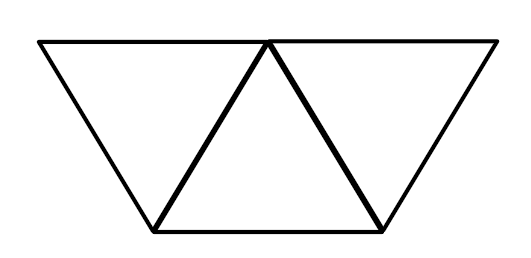
\includegraphics{Discrete/matrix_graf_incorrect.PNG}}
\end{flaw}

\clearpage
\subsection{Error classification}

%Provide a brief classification and explanation of the errors in the Flawed Proof \ref{flaw:proof1}. %change the label

There are several errors
% is only one error ... etc.
 in the Flawed Proof \ref{flaw:matrix_graf}. %change the label

 
 \begin{description}
 	\item[N-N:] The vertices $v_1, ..., v_5$ are not labeled, which makes it difficult to interpret the graph. 
 	\item[N-VG:] There are no explanations provided; more detail is required. 
 \end{description}

 
\subsubsection{Error codes}
\begin{itemize}
	\item 	Novice Notation (N-N)
	\item   Novice Vocabulary and Grammar (N-VG)
\end{itemize}
See Section \ref{sec-error} for more information about error classifications.

\clearpage
\subsection{Corrected proof}

The following is a corrected version of Flawed Proof \ref{flaw:matrix_graf}. %change the label

\begin{prf}{prf:matrix_graf} %change the label
\center{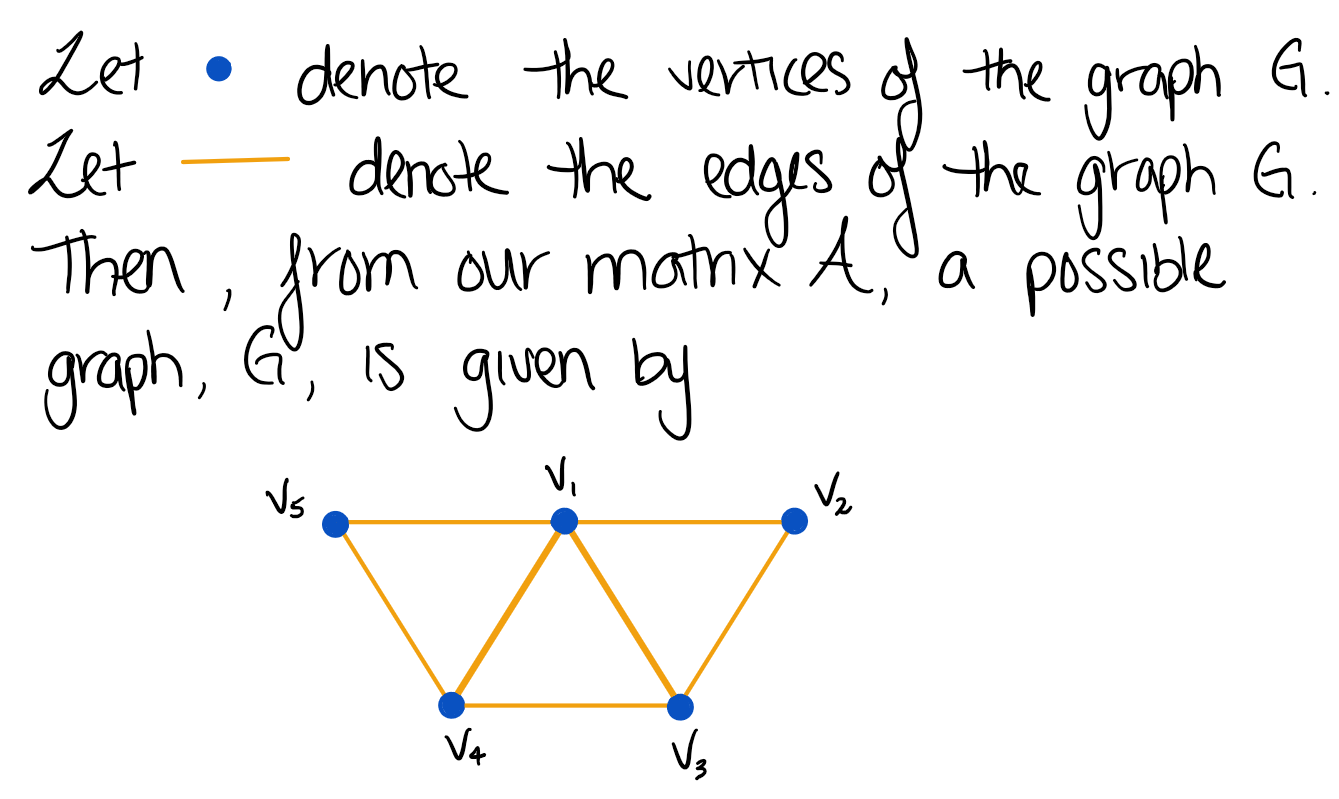
\includegraphics{Discrete/matrix_graf_correct.PNG}}
\end{prf}